\documentclass[12pt,a4paper,oneside]{report}

% =========================
% Encoding, Language, Fonts
% =========================
\usepackage{fontspec}
\IfFontExistsTF{Times New Roman}
  {\setmainfont{Times New Roman}}
  {\setmainfont{TeX Gyre Termes}}
\usepackage[vietnamese]{babel}

% =========================
% Page Layout and Styling
% =========================
\usepackage[a4paper,top=2.5cm,bottom=2.5cm,left=3.0cm,right=2.5cm]{geometry}
\usepackage{setspace}
\setstretch{1.25}
\newlength{\manualparindent}
\setlength{\manualparindent}{1.2cm}
\setlength{\parindent}{0pt}
\setlength{\parskip}{0.08em}
\newcommand{\manualindent}{\hspace*{\manualparindent}}
\sloppy

\usepackage{tikz}
\usepackage{xcolor}
\usepackage{graphicx}
\usepackage{float}
\usepackage{booktabs}
\usepackage{longtable}
\usepackage{array}
\usepackage{tabularx}
\usepackage{multirow}
\usepackage{amsmath,amssymb}
\usepackage{enumitem}
\usepackage{listings}
\usepackage{caption}
\usepackage{titlesec}
\usepackage[hidelinks]{hyperref}

\setlist{topsep=0.25em,itemsep=0.1em,parsep=0pt}
\titlespacing*{\chapter}{0pt}{-0.4cm}{0.8cm}
\titlespacing*{\section}{0pt}{0.7em}{0.35em}
\titlespacing*{\subsection}{0pt}{0.5em}{0.25em}

\graphicspath{{./}{../documents/}{../documents/paper-assets/}{../cs106/evaluation/eval_outputs/}}

\definecolor{uitblue}{RGB}{0,65,120}
\definecolor{lightgray}{RGB}{245,245,245}
\definecolor{darkgray}{RGB}{60,60,60}

\newcommand{\coverborder}{%
  \begin{tikzpicture}[remember picture,overlay]
    \draw[line width=0.8pt]
      ([xshift=1.2cm,yshift=-1.2cm]current page.north west)
      rectangle
      ([xshift=-1.2cm,yshift=1.2cm]current page.south east);
    \draw[line width=0.3pt]
      ([xshift=1.35cm,yshift=-1.35cm]current page.north west)
      rectangle
      ([xshift=-1.35cm,yshift=1.35cm]current page.south east);
  \end{tikzpicture}
}

\newcommand{\universitylogo}{%
  \IfFileExists{uit.png}{%
    
\includegraphics[height=2.7cm]{uit.png}%
  }{%
    \begin{tikzpicture}
      \draw[line width=0.6pt, color=uitblue] (0,0) rectangle (3.2,2.6);
      \node[align=center, color=uitblue, font=\bfseries\small] at (1.6,1.3)
      {LOGO\\UIT};
    \end{tikzpicture}%
  }%
}

\newcommand{\placeholderfigure}[1]{%
  \fbox{\begin{minipage}{0.88\textwidth}
    \centering
    \vspace{0.3cm}
    \textit{#1}
    \vspace{0.3cm}
  \end{minipage}}%
}

\captionsetup{
  font=small,
  labelfont=bf,
  justification=centering
}

\lstdefinestyle{promptstyle}{
  basicstyle=\ttfamily\small,
  backgroundcolor=\color{lightgray},
  frame=single,
  breaklines=true,
  columns=fullflexible,
  keepspaces=true,
  showstringspaces=false
}

\renewcommand{\contentsname}{MỤC LỤC}
\renewcommand{\chaptername}{Chương}
\renewcommand{\bibname}{TÀI LIỆU THAM KHẢO}
\renewcommand{\figurename}{Hình}
\renewcommand{\tablename}{Bảng}

\newcommand{\projecttitle}{TÁI HIỆN VÀ ĐÁNH GIÁ KHẢ NĂNG SUY LUẬN CỦA LLM THÔNG QUA SUDOKU-BENCH}

\begin{document}

% =========================
% Cover Page
% =========================
\begin{titlepage}
  \begingroup
  \setstretch{1.0}
  \setlength{\parskip}{0pt}
  \coverborder
  \centering
  \vspace*{0.35cm}

  {\bfseries\Large TRƯỜNG ĐẠI HỌC CÔNG NGHỆ THÔNG TIN}\\
  {\bfseries\large ĐẠI HỌC QUỐC GIA THÀNH PHỐ HỒ CHÍ MINH}\\
  {\bfseries\large KHOA KHOA HỌC MÁY TÍNH}

  \vspace{0.45cm}
  \IfFileExists{uit.png}{
\includegraphics[height=2.1cm]{uit.png}}{\universitylogo}

  \vspace{0.6cm}

  {\bfseries\Large BÁO CÁO ĐỒ ÁN CUỐI KỲ}\\[0.25cm]
  {\bfseries\large MÔN HỌC: CS106 - TRÍ TUỆ NHÂN TẠO}

  \vspace{0.85cm}

  \begin{minipage}{0.9\textwidth}
    \centering
    {\bfseries\large\color{uitblue} \projecttitle}
  \end{minipage}

  \vspace{0.85cm}

  \small
  \begin{tabular}{>{\bfseries}p{4.6cm}p{8.2cm}}
    Giảng viên hướng dẫn: & Lương Ngọc Hoàng \\
    Nhóm thực hiện: & Nhóm 4 \\
    Bài báo tham chiếu: & Sudoku-Bench: Evaluating Creative Reasoning with Sudoku Variants \\
    Thời gian thực hiện: & 05/2026 \\
  \end{tabular}

  \vspace{0.55cm}

  \begin{tabular}{clc}
    \toprule
    STT & Họ và tên & MSSV \\
    \midrule
    1 & Phan Công Nam & 23520986 \\
    2 & Đặng Anh Khoa & 23520732 \\
    3 & Phạm Minh Bảo Khang & 23520705 \\
    4 & Nguyễn Khang Hy & 23520662 \\
    \bottomrule
  \end{tabular}

  \vspace{0.6cm}
  {\bfseries TP. Hồ Chí Minh, tháng 05 năm 2026}
  \endgroup
\end{titlepage}

\pagenumbering{roman}
\tableofcontents
\clearpage
\pagenumbering{arabic}

% =========================
% Abstract
% =========================
\chapter*{TÓM TẮT}
\addcontentsline{toc}{chapter}{TÓM TẮT}

\manualindent%
Đồ án này nghiên cứu khả năng suy luận logic của các mô hình ngôn ngữ lớn (Large Language Models -- LLMs) thông qua việc tái hiện một phần bài báo \textit{Sudoku-Bench: Evaluating Creative Reasoning with Sudoku Variants}. Thay vì kiểm tra mô hình bằng các tác vụ ngôn ngữ quen thuộc, Sudoku-Bench dùng các biến thể Sudoku có luật chặt chẽ, nghiệm kiểm chứng được và yêu cầu suy luận nhiều bước. Đây là môi trường phù hợp để đánh giá liệu LLM có thật sự duy trì được trạng thái logic nhất quán hay chỉ sinh ra lời giải nghe có vẻ hợp lý.

\manualindent%
Trong phạm vi đồ án, nhóm tập trung vào biến thể Killer Sudoku. Nhóm xây dựng pipeline đánh giá tự động gồm: đọc dữ liệu JSON, tạo prompt từ luật và trạng thái lưới, gọi API Gemini, parse phản hồi, validate với nghiệm chuẩn, lưu output và tổng hợp kết quả bằng notebook evaluation. Thực nghiệm được tiến hành trên 5 bài Killer Sudoku 6x6 easy và 2 bài Killer Sudoku 9x9 hard, với bốn mô hình Gemini: Gemini 2.5 Flash, Gemini 2.5 Pro, Gemini 3.1 Flash Lite và Gemini 3.5 Flash. Nhóm đánh giá cả hai chế độ single-prompt và multi-step.

\manualindent%
Kết quả cho thấy 6x6 easy là mức mà các mô hình mạnh có thể xử lý tốt: Gemini 2.5 Pro và Gemini 3.5 Flash đạt 100\% ở single-prompt 6x6, còn Gemini 3.5 Flash đạt 100\% ở multi-step 6x6. Khi mở rộng sang 9x9 hard, single-prompt giảm mạnh: chỉ Gemini 3.5 Flash giải được 1/2 bài. Ngược lại, multi-step giúp Gemini 2.5 Pro và Gemini 3.5 Flash giải đúng cả 2/2 bài 9x9, trong khi các mô hình yếu hơn bị kẹt ở lỗi \textit{No Certain Move}. Kết quả này phù hợp với tinh thần của Sudoku-Bench: các bài lớn và giàu ràng buộc giúp bộc lộ rõ hơn giới hạn của LLM trong suy luận dài hạn.

\manualindent%
\textbf{Từ khóa:} Sudoku-Bench, Killer Sudoku, Large Language Models, logical reasoning, multi-step reasoning, evaluation benchmark.

% =========================
% Chapter 1
% =========================
\chapter{TỔNG QUAN}

\section{Bối cảnh và lý do chọn đề tài}

\manualindent%
Các mô hình ngôn ngữ lớn hiện nay thể hiện năng lực ấn tượng trong nhiều tác vụ như trả lời câu hỏi, sinh văn bản, hỗ trợ lập trình và giải thích kiến thức. Tuy nhiên, thành công trên các tác vụ ngôn ngữ không đồng nghĩa với việc mô hình có khả năng suy luận logic một cách bền vững. Một câu trả lời có thể nghe hợp lý nhưng vẫn sai về mặt hình thức, đặc biệt trong các bài toán có ràng buộc nghiêm ngặt.

\manualindent%
Trong các bài toán thỏa mãn ràng buộc, mỗi quyết định trung gian phải nhất quán với toàn bộ trạng thái hiện tại. Một bước sai có thể làm cho các bước sau trở nên vô nghĩa, dù phần giải thích vẫn có vẻ thuyết phục. Đây là điểm khác biệt quan trọng giữa \textit{sinh lập luận} và \textit{duy trì một lời giải đúng}. Vì vậy, cần có các benchmark mà kết quả cuối có thể được kiểm chứng khách quan.

\manualindent%
Sudoku và các biến thể Sudoku là môi trường phù hợp cho mục tiêu này. Một lời giải Sudoku không chỉ cần đầy đủ mà còn phải đồng thời thỏa mãn luật hàng, cột, vùng và các ràng buộc bổ sung. Đặc biệt, các Sudoku variants thường có lưới ban đầu rất ít dữ kiện, buộc người giải phải tìm ra các điểm đột phá logic ban đầu, hay còn gọi là \textit{break-in}. Bài báo Sudoku-Bench khai thác đặc điểm này để đánh giá năng lực suy luận sáng tạo của LLM \cite{sudoku-bench}.

\section{Mục tiêu đồ án}

Đồ án có bốn mục tiêu chính:

\begin{enumerate}[label=\arabic*.]
  \item Trình bày lý thuyết liên quan đến Sudoku variants, Killer Sudoku, suy luận logic nhiều bước và thiết kế benchmark trong bài báo Sudoku-Bench.
  \item Tái hiện một phần quy trình đánh giá của bài báo bằng một pipeline thực nghiệm có thể đọc đề, gọi LLM, parse phản hồi và validate tự động.
  \item Benchmark nhiều mô hình Gemini trên hai chế độ single-prompt và multi-step, với dữ liệu 6x6 và 9x9.
  \item Phân tích kết quả, phân loại lỗi, so sánh với tinh thần của bài báo gốc và nêu giới hạn của thực nghiệm trong phạm vi đồ án.
\end{enumerate}

\section{Phạm vi và đóng góp}

\manualindent%
Trọng tâm của đồ án là thuyết trình và tái hiện một phần bài báo tham chiếu, không bắt buộc phải xây dựng một thuật toán CSP thuần túy. Vì vậy, nhóm không cài đặt solver Sudoku truyền thống để giải hộ mô hình. Các khái niệm về ràng buộc chỉ được dùng như nền tảng lý thuyết để giải thích vì sao Sudoku variants là một benchmark phù hợp cho LLM. Trong thực nghiệm, mô hình nhận luật và trạng thái bài toán bằng ngôn ngữ, sau đó phải tự đưa ra lời giải hoặc bước đi. Hệ thống của nhóm chỉ đóng vai trò tạo prompt, ghi log và kiểm chứng kết quả.

Phạm vi thực nghiệm gồm:

\begin{itemize}
  \item Biến thể chính: Killer Sudoku.
  \item Dataset: 5 bài 6x6 easy và 2 bài 9x9 hard.
  \item Mô hình: Gemini 2.5 Flash, Gemini 2.5 Pro, Gemini 3.1 Flash Lite và Gemini 3.5 Flash.
  \item Chế độ: single-prompt và multi-step.
  \item Đánh giá: solve rate, final status, error type, average correct placements, số bước và thời gian chạy single-prompt.
\end{itemize}

Đóng góp của nhóm nằm ở việc tái hiện rút gọn một benchmark nghiên cứu, xây dựng pipeline đánh giá có validator và log, đồng thời phân tích thực nghiệm theo nhiều kích thước lưới và nhiều mức năng lực mô hình.

\section{Cấu trúc báo cáo}

\manualindent%
Phần còn lại của báo cáo được tổ chức như sau. Chương 2 trình bày cơ sở lý thuyết trong bài báo: Sudoku variants, Killer Sudoku, break-in và góc nhìn ràng buộc. Chương 3 tóm tắt bài báo Sudoku-Bench và so sánh phạm vi tái hiện của nhóm với bài báo gốc. Chương 4 mô tả dataset, pipeline và thiết kế thực nghiệm. Chương 5 trình bày kết quả benchmark và phân tích lỗi. Chương 6 kết luận, nêu hạn chế và hướng phát triển.

% =========================
% Chapter 2
% =========================
\chapter{CƠ SỞ LÝ THUYẾT}

\section{Sudoku dưới góc nhìn ràng buộc}

\manualindent%
Sudoku có thể được nhìn như một bài toán thỏa mãn ràng buộc (Constraint Satisfaction Problem -- CSP). Cách nhìn này giúp giải thích vì sao Sudoku variants là môi trường tốt để đánh giá reasoning của LLM, nhưng không đồng nghĩa với việc đồ án phải xây dựng một solver CSP. Một bài toán thỏa mãn ràng buộc thường được mô hình hóa bởi bộ ba:

\[
  \langle X, D, C \rangle
\]

\manualindent%
Trong đó \(X = \{X_1, X_2, ..., X_n\}\) là tập biến, \(D = \{D_1, D_2, ..., D_n\}\) là miền giá trị tương ứng của các biến, và \(C\) là tập ràng buộc xác định các tổ hợp giá trị hợp lệ. Mục tiêu là tìm một phép gán giá trị cho toàn bộ biến sao cho tất cả ràng buộc đều được thỏa mãn \cite{russell-norvig}.

\manualindent%
Sudoku chuẩn là ví dụ trực quan của CSP. Mỗi ô trên lưới là một biến; miền giá trị là các chữ số hợp lệ; ràng buộc là điều kiện không lặp số trong từng hàng, cột và vùng. Với Sudoku 9x9, mỗi ô nhận giá trị từ 1 đến 9; với Sudoku 6x6, mỗi ô nhận giá trị từ 1 đến 6.

\manualindent%
Các thuật toán truyền thống thường kết hợp tìm kiếm và lan truyền ràng buộc, chẳng hạn backtracking hoặc forward checking. Tuy nhiên, trong đồ án này, nhóm không dùng các kỹ thuật đó để tạo lời giải. Điểm cần nhấn mạnh là: paper Sudoku-Bench dùng Sudoku variants để đánh giá khả năng mô hình tự đọc luật, tự suy luận và tự duy trì tính nhất quán logic.

\section{Sudoku variants}

\manualindent%
Sudoku variants mở rộng Sudoku chuẩn bằng cách bổ sung các luật ngoài hàng, cột và vùng. Các luật này có thể dựa trên quan hệ hình học, tổng số, thứ tự, đường đi hoặc điều kiện meta. Ví dụ:

\begin{itemize}
  \item \textbf{Knight's Move}: hai ô cách nhau như nước đi quân mã không được có cùng chữ số.
  \item \textbf{Arrow}: tổng các ô trên thân mũi tên bằng giá trị ở vòng tròn gốc.
  \item \textbf{Thermometer}: chữ số tăng dần dọc theo nhiệt kế.
  \item \textbf{Killer Cage}: các ô trong cage không lặp và có tổng bằng giá trị cho trước.
\end{itemize}

Điểm quan trọng của Sudoku variants là luật có thể được mô tả bằng ngôn ngữ tự nhiên. Điều này làm cho bài toán phù hợp với LLM: mô hình phải đọc hiểu luật, chuyển luật thành ràng buộc và áp dụng vào từng trạng thái lưới.

\section{Killer Sudoku}

\manualindent%
Killer Sudoku kết hợp luật Sudoku chuẩn với các cage. Mỗi cage gồm một nhóm ô và một tổng mục tiêu. Các chữ số trong cùng cage không được lặp và tổng của chúng phải bằng tổng mục tiêu. Ví dụ, trong lưới 6x6, nếu cage gồm hai ô có tổng bằng 3 thì hai ô đó chỉ có thể là cặp \(\{1,2\}\), nhưng vẫn cần kết hợp với hàng, cột và vùng để xác định ô nào là 1 và ô nào là 2.

\manualindent%
Ràng buộc cage tạo ra các phương trình số học cục bộ, nhưng lời giải cuối vẫn phụ thuộc vào tính nhất quán toàn cục. Đây là điểm khiến Killer Sudoku phù hợp để đánh giá LLM: mô hình phải vừa tính tổ hợp số, vừa duy trì trạng thái của nhiều hàng, cột, vùng và cage.

\section{Break-in và suy luận sáng tạo}

\manualindent%
Nhiều Sudoku variants không thể bắt đầu bằng một bước hiển nhiên. Người giải cần tìm một \textit{break-in}: một điểm suy luận ban đầu giúp thu hẹp không gian nghiệm và mở khóa các bước tiếp theo. Break-in thường xuất hiện từ tương tác tinh tế giữa nhiều ràng buộc, chứ không chỉ từ một luật đơn lẻ.

\manualindent%
Theo Sudoku-Bench, chính yêu cầu tìm break-in làm cho Sudoku variants trở thành benchmark tốt cho creative reasoning. Mô hình không thể chỉ dựa vào mẫu Sudoku chuẩn; nó phải hiểu luật mới và phát hiện cách các luật kết hợp với nhau.

\section{Giới hạn của LLM trong suy luận ràng buộc}

\manualindent%
LLM sinh phản hồi theo cơ chế tự hồi quy: mỗi token được sinh dựa trên ngữ cảnh trước đó. Cơ chế này mạnh trong các tác vụ ngôn ngữ, nhưng không đảm bảo duy trì một trạng thái ràng buộc chính xác như một solver hình thức. Một mô hình có thể trình bày lập luận nghe hợp lý nhưng vẫn bỏ sót một ràng buộc hoặc nhầm lẫn giữa \textit{ứng viên có thể} và \textit{giá trị bắt buộc}.

\manualindent%
Trong bối cảnh Sudoku, lỗi nhỏ này rất nghiêm trọng. Nếu mô hình điền sai một ô, toàn bộ lời giải sau đó có thể bị kéo lệch. Vì vậy, đánh giá LLM trên Sudoku cần có validator độc lập và metric rõ ràng thay vì chỉ đọc phần reasoning bằng mắt.

% =========================
% Chapter 3
% =========================
\chapter{BÀI BÁO THAM CHIẾU SUDOKU-BENCH}

\section{Mục tiêu của bài báo}

\manualindent%
Bài báo \textit{Sudoku-Bench: Evaluating Creative Reasoning with Sudoku Variants} đề xuất một benchmark nhằm đánh giá năng lực creative reasoning của LLM trên các Sudoku variants \cite{sudoku-bench}. Tác giả lập luận rằng nhiều benchmark reasoning phổ biến có thể bị ảnh hưởng bởi việc mô hình đã học các mẫu giải quen thuộc. Sudoku variants giảm rủi ro này vì mỗi puzzle có sự kết hợp luật riêng, thường yêu cầu suy luận mới và break-in không hiển nhiên.

Benchmark này có ba đặc điểm đáng chú ý:

\begin{itemize}
  \item Các puzzle có nghiệm duy nhất và có thể kiểm chứng.
  \item Luật puzzle được mô tả bằng ngôn ngữ tự nhiên và có thể chuẩn hóa thành text representation.
  \item Bài toán đủ khó để phân tách các mô hình hiện đại, đặc biệt ở kích thước lớn và luật phức tạp.
\end{itemize}

\section{Thiết kế benchmark trong bài báo}

\manualindent%
Sudoku-Bench gồm 100 Sudoku variants được tuyển chọn, bao phủ nhiều loại ràng buộc và nhiều mức độ khó. Bài báo cung cấp công cụ biểu diễn puzzle bằng văn bản để tách phần suy luận logic khỏi phần nhận dạng hình ảnh. Đây là điểm quan trọng vì mục tiêu chính là kiểm tra reasoning, không phải thị giác máy tính.

Bài báo đánh giá mô hình trong hai chế độ:

\begin{itemize}
  \item \textbf{Single-shot}: mô hình nhận toàn bộ puzzle và trả về lời giải hoàn chỉnh trong một lần.
  \item \textbf{Multi-step}: mô hình tương tác qua nhiều lượt, mỗi lượt đưa ra ít nhất một chữ số; hệ thống cập nhật trạng thái và tiếp tục.
\end{itemize}

Kết quả baseline trong bài báo cho thấy ngay cả các mô hình mạnh cũng giải được ít hơn 15\% puzzle khi không có công cụ hỗ trợ. Hiệu năng giảm mạnh ở các puzzle lớn hơn và ít quen thuộc hơn. Đây là động lực trực tiếp cho đồ án: kiểm tra lại hiện tượng này trong phạm vi nhỏ hơn, có kiểm soát hơn.

\section{Phạm vi tái hiện của nhóm}

\manualindent%
Nhóm không tái hiện toàn bộ 100 puzzle và toàn bộ tập model của bài báo. Thay vào đó, nhóm chọn Killer Sudoku làm biến thể chính và xây dựng một pipeline riêng để tái hiện tinh thần đánh giá.

\begin{table}[H]
  \centering
  \caption{So sánh bài báo gốc và phạm vi đồ án}
  \small
  \begin{tabularx}{\textwidth}{p{3.1cm}XX}
    \toprule
    Tiêu chí & Sudoku-Bench & Đồ án của nhóm \\
    \midrule
    Mục tiêu & Đánh giá creative reasoning của LLM trên Sudoku variants & Tái hiện rút gọn việc đánh giá suy luận ràng buộc của LLM trên Killer Sudoku \\
    Dữ liệu & 100 puzzle tuyển chọn, nhiều variant và mức khó & 5 puzzle 6x6 easy, 2 puzzle 9x9 hard \\
    Biến thể & Nhiều luật như arrow, thermometer, knight move, killer, meta-constraints & Tập trung Killer Sudoku để kiểm soát phạm vi \\
    Biểu diễn & Text representation chuẩn hóa, có công cụ tương tác SudokuPad & JSON nội bộ gồm grid, solution, cages và prompt text \\
    Chế độ & Single-shot và multi-step & Single-prompt và multi-step \\
    Model & Nhiều LLM thương mại/mã nguồn mở & 4 model Gemini \\
    Đánh giá & Solve rate, lỗi, phân tích quá trình & Solve rate, status, error type, correct placements, thời gian single-prompt \\
    \bottomrule
  \end{tabularx}
\end{table}

\manualindent%
Việc rút gọn là cần thiết vì multi-step rất tốn chi phí: với lưới 6x6 có 36 ô, một phiên giải có thể cần khoảng 72 lượt gọi nếu mỗi ô gồm một bước analysis và một bước fill; với 9x9, con số tối thiểu có thể lên tới 162 lượt gọi. Vì vậy, nhóm ưu tiên tập nhỏ nhưng có log và đánh giá chi tiết.

\section{Các chỉ số đánh giá}

Chỉ số quan trọng nhất là solve rate:

\[
  \text{Solve Rate} = \frac{\text{số puzzle giải đúng hoàn toàn}}{\text{tổng số puzzle}}
\]

Tuy nhiên, solve rate chỉ cho biết mô hình có hoàn thành puzzle hay không. Đối với multi-step, nhóm dùng thêm \textit{average correct placements}, tức số ô trung bình mà mô hình đã điền đúng trước khi phiên chạy kết thúc. Metric này giúp phân biệt hai mô hình cùng 0\% solve rate nhưng một mô hình đi được nhiều bước đúng hơn trước khi bị kẹt hoặc sai.

Nhóm cũng ghi nhận \textit{error type}. Trong thực nghiệm hiện tại có hai nhóm lỗi chính:

\begin{itemize}
  \item \textbf{Incorrect Solution}: mô hình đưa ra nghiệm hoặc bước đi sai.
  \item \textbf{No Certain Move}: mô hình không tìm được bước chắc chắn để tiếp tục.
\end{itemize}

% =========================
% Chapter 4
% =========================
\chapter{PHƯƠNG PHÁP THỰC NGHIỆM}

\section{Dữ liệu thực nghiệm}

\manualindent%
Dataset của nhóm gồm 7 puzzle Killer Sudoku. Các puzzle được lưu trong thư mục dataset dưới dạng JSON, mỗi file gồm mã puzzle, kích thước lưới, độ khó, board ban đầu, nghiệm chuẩn và danh sách cage.

\begin{table}[H]
  \centering
  \caption{Tập dữ liệu thực nghiệm}
  \begin{tabular}{ccccc}
    \toprule
    Puzzle & Kích thước & Độ khó & Số cage & Vai trò \\
    \midrule
    1 & 6x6 & easy & 14 & Tập chính \\
    2 & 6x6 & easy & 16 & Tập chính \\
    3 & 6x6 & easy & 16 & Tập chính \\
    4 & 6x6 & easy & 15 & Tập chính \\
    5 & 6x6 & easy & 15 & Tập chính \\
    6 & 9x9 & hard & 29 & Stress-test \\
    7 & 9x9 & hard & 33 & Stress-test \\
    \bottomrule
  \end{tabular}
\end{table}

\manualindent%
Nhóm không dùng 4x4 làm tập chính vì kích thước này quá nhỏ và dễ bị giải trọn vẹn bằng single-prompt, khó tạo khác biệt rõ giữa các mô hình. Ngược lại, 9x9 có chi phí cao nên chỉ dùng 2 puzzle hard để kiểm tra khả năng mở rộng.

\section{Mô hình được đánh giá}

\begin{table}[H]
  \centering
  \caption{Các mô hình trong thực nghiệm}
  \begin{tabularx}{\textwidth}{p{4.2cm}X}
    \toprule
    Mô hình & Vai trò trong thực nghiệm \\
    \midrule
    Gemini 2.5 Flash & Model nhanh, chi phí thấp hơn, dùng làm baseline thực dụng \\
    Gemini 2.5 Pro & Model mạnh hơn trong dòng 2.5, kỳ vọng suy luận tốt hơn \\
    Gemini 3.1 Flash Lite & Model nhẹ hơn, dùng như baseline yếu \\
    Gemini 3.5 Flash & Model mới/mạnh hơn trong tập thử nghiệm, dùng để kiểm tra cải thiện hiệu năng \\
    \bottomrule
  \end{tabularx}
\end{table}

\manualindent%
Các lượt gọi được cấu hình với nhiệt độ thấp để giảm tính ngẫu nhiên. Output được yêu cầu ở dạng JSON để parser có thể xử lý tự động.

\section{Single-prompt evaluation}

\manualindent%
Ở chế độ single-prompt, mô hình nhận toàn bộ luật, board ban đầu, danh sách cage và cheat sheet trong một prompt duy nhất. Mô hình phải trả về một grid hoàn chỉnh. Parser đọc grid này và validator so sánh trực tiếp với nghiệm chuẩn. Chế độ này có ưu điểm là ít lượt gọi API và thời gian chạy thấp hơn, nhưng khi mô hình fail, hệ thống khó biết lỗi xuất hiện ở bước suy luận nào.

\section{Multi-step evaluation}

Ở chế độ multi-step, mô hình không trả lời toàn bộ grid ngay lập tức. Mỗi vòng gồm hai giai đoạn:

\begin{enumerate}[label=\arabic*.]
  \item \textbf{Analysis}: mô hình phân tích trạng thái hiện tại, các ràng buộc và ứng viên.
  \item \textbf{Fill}: mô hình chọn đúng một ô để điền, trả về ô, giá trị, reasoning và trạng thái chắc chắn.
\end{enumerate}

Sau mỗi bước fill, board được cập nhật và validator kiểm tra ngay. Nếu mô hình điền sai, phiên chạy dừng. Nếu mô hình không tìm được bước chắc chắn, phiên chạy cũng dừng với lỗi No Certain Move. Thiết kế này tuân thủ nguyên tắc: hệ thống không giải hộ mô hình, chỉ cung cấp ngữ cảnh, cập nhật trạng thái và kiểm tra đúng/sai.

\clearpage
\section{Định dạng output và validator}

Một phản hồi fill hợp lệ có dạng:

\begin{lstlisting}[style=promptstyle]
{
  "reasoning": "Subgrid 3 must sum to 21...",
  "cell": "r3c3",
  "value": 2,
  "is_certain": true
}
\end{lstlisting}

Validator kiểm tra:

\begin{itemize}
  \item Ô được chọn có nằm trong board và còn trống không;
  \item Giá trị có nằm trong miền hợp lệ không;
  \item Giá trị có khớp với nghiệm chuẩn không;
  \item Trạng thái hiện tại có còn nhất quán với nghiệm chuẩn không;
  \item Grid cuối có giải đúng hoàn toàn không.
\end{itemize}

\section{Cheat sheet Killer Sudoku}

\manualindent%
Cheat sheet cung cấp các tổ hợp cage hợp lệ theo kích thước cage và tổng mục tiêu. Ví dụ, với lưới 6x6, một cage 2 ô có tổng 3 chỉ có thể là \(\{1,2\}\). Cheat sheet không chỉ ra ô nào nhận giá trị nào và không chứa nghiệm của puzzle. Vai trò của nó là giảm lỗi tính toán tổ hợp cơ bản, để mô hình tập trung hơn vào việc kết hợp nhiều ràng buộc.

\section{Pipeline tổng quát}

\begin{figure}[H]
  \centering
  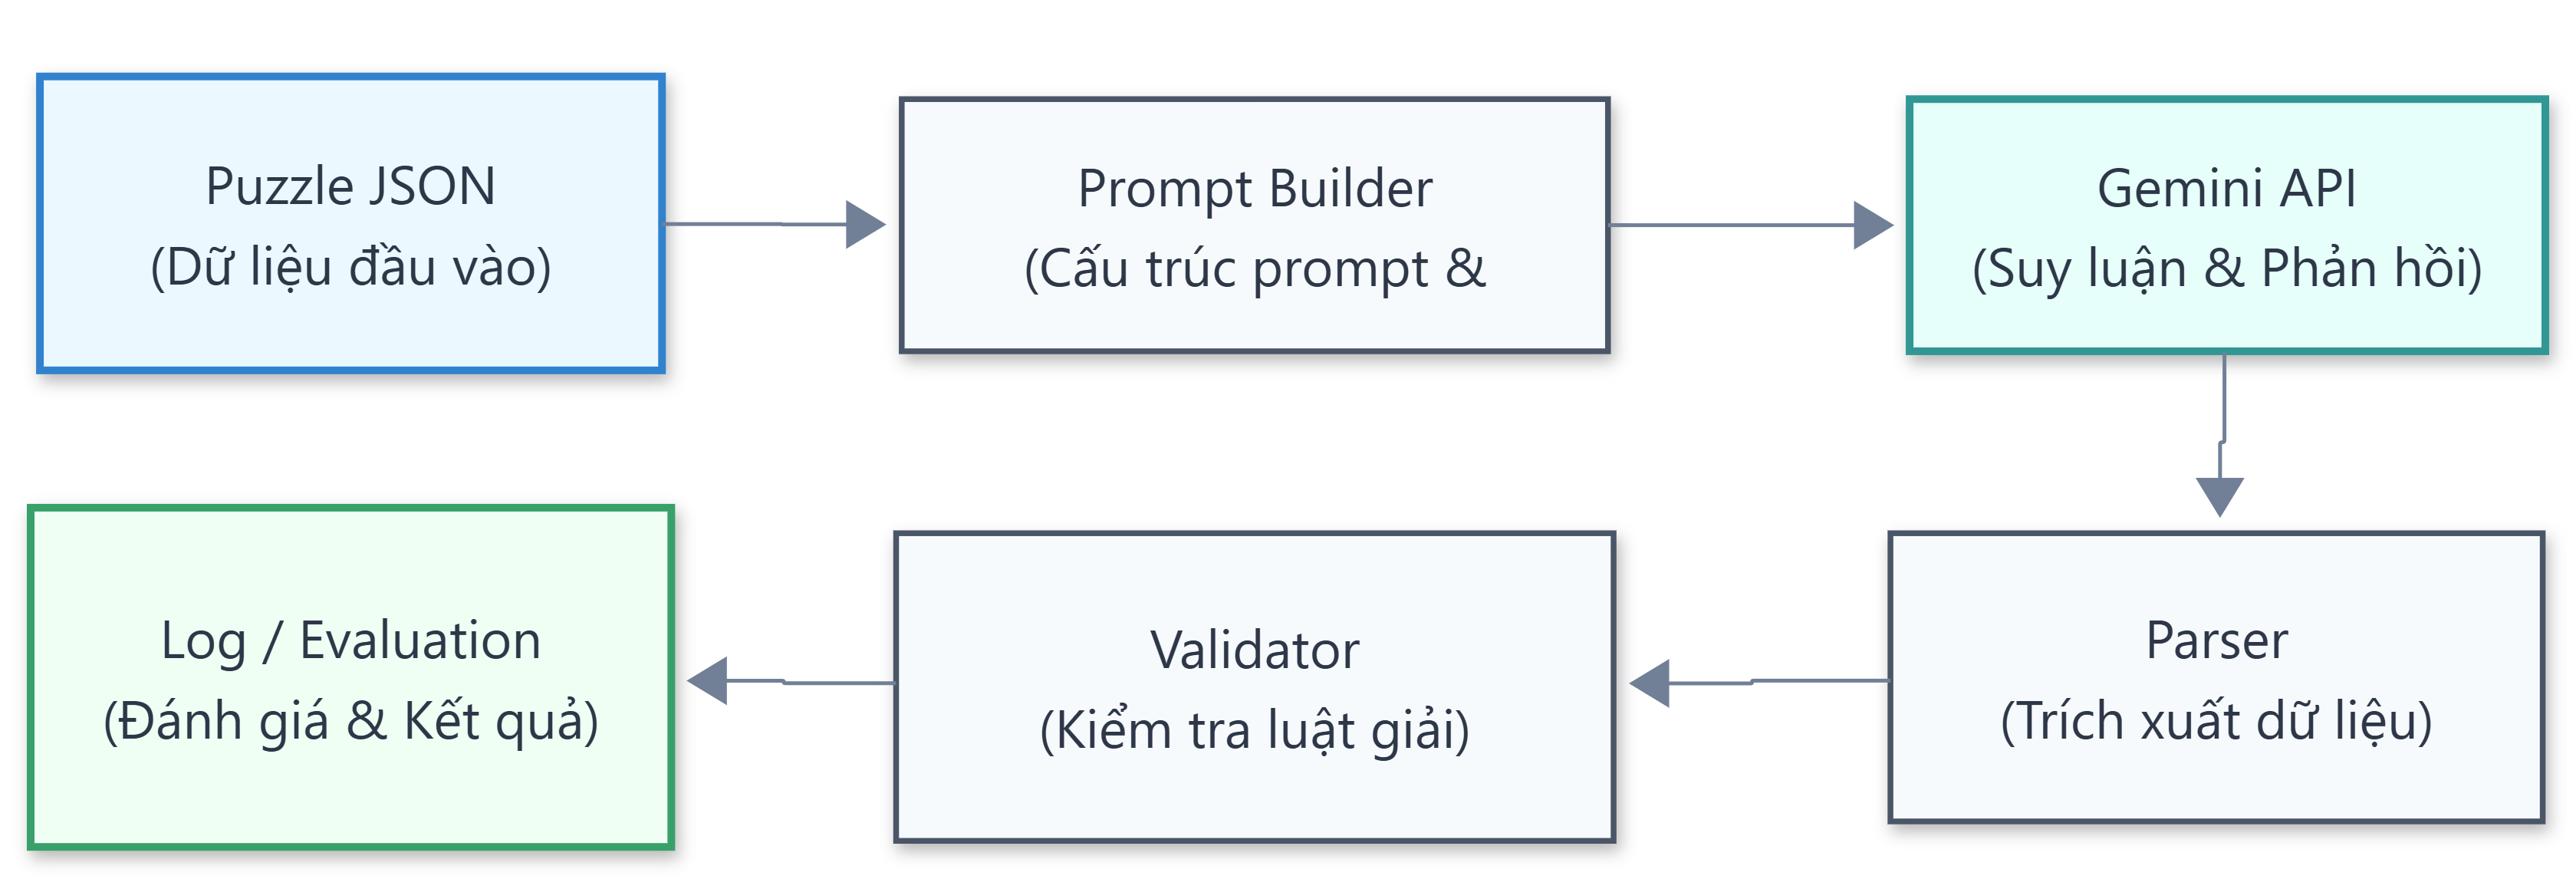
\includegraphics[width=0.95\textwidth]{Pipeline-danh-gia.png}
  \caption{Pipeline đánh giá của nhóm}
\end{figure}

\manualindent%
Kết quả cuối được lưu thành JSON log hoặc result JSON, sau đó notebook evaluation tổng hợp thành các file CSV và biểu đồ.

\section{Các thành phần cài đặt quan trọng}

\subsection{Cấu trúc prompt}

\manualindent%
Prompt được xây dựng từ dữ liệu puzzle và trạng thái hiện tại của board. Với single-prompt, toàn bộ thông tin được đưa vào một lần; với multi-step, prompt được cập nhật sau mỗi bước đi. Cấu trúc rút gọn như sau:

\begin{lstlisting}[style=promptstyle]
System / instruction:
  - You are solving Killer Sudoku.
  - Follow normal Sudoku rules.
  - Follow cage sum rules.
  - Do not guess.

Puzzle context:
  - grid size
  - current board
  - list of cages: sum + cells
  - Killer Sudoku cheat sheet

Output requirement:
  - single-prompt: return a complete grid
  - multi-step fill: return exactly one cell as JSON
\end{lstlisting}

\manualindent%
Thiết kế này giúp tách rõ ba loại thông tin: luật chung, dữ liệu cụ thể của puzzle và định dạng output bắt buộc. Nhờ đó parser có thể xử lý phản hồi tự động thay vì đọc thủ công.

\subsection{Vòng lặp multi-step}

\manualindent%
Trong multi-step, mô hình không được trả về toàn bộ nghiệm ngay lập tức mà phải đi từng bước. Pseudo-code của vòng lặp chính như sau:

\begin{lstlisting}[style=promptstyle]
current_board = initial_board

while board is valid and not fully filled:
    analysis = call_llm_analysis(current_board, cages, cheat_sheet)
    move = call_llm_fill(current_board, cages, analysis)

    if move.is_certain is false:
        return Failed("No Certain Move")

    if move.cell is invalid or already filled:
        return Failed("Invalid Move")

    update current_board with move

    if current_board differs from solution at any filled cell:
        return Failed("Incorrect Solution")

return Success
\end{lstlisting}

\manualindent%
Điểm quan trọng là validator chạy ngay sau mỗi bước fill. Do đó nếu mô hình sai, phiên chạy dừng tại bước sai đầu tiên thay vì để mô hình tiếp tục xây dựng reasoning trên một trạng thái đã sai.

\subsection{Validator}

\manualindent%
Validator là thành phần cốt lõi của pipeline vì nó tách phần đánh giá khỏi phần sinh câu trả lời của LLM. Validator không gợi ý bước đi, không loại ứng viên và không sửa lỗi cho mô hình. Nó chỉ kiểm tra phản hồi sau khi mô hình đã đưa ra quyết định.

\begin{lstlisting}[style=promptstyle]
function validate_current_state(solution, current_board):
    for each cell (r, c):
        if current_board[r][c] is empty:
            continue
        if current_board[r][c] != solution[r][c]:
            return false
    return true

function is_all_filled(board):
    return every cell is non-empty
\end{lstlisting}

\manualindent%
Với single-prompt, validator so sánh toàn bộ prediction grid với solution grid. Với multi-step, validator kiểm tra từng trạng thái trung gian. Cách làm này giúp báo cáo không phụ thuộc vào việc người đọc có thấy reasoning của mô hình hợp lý hay không; kết quả được quyết định bằng nghiệm chuẩn.

\clearpage
\subsection{Parser và chuẩn hóa output}

\manualindent%
Do LLM có thể sinh thêm giải thích ngoài JSON, parser cần chuẩn hóa phản hồi trước khi validate. Ở các phiên mới, nhóm ưu tiên cấu hình response schema hoặc yêu cầu \texttt{response\_mime\_type = application/json}. Logic parser có thể tóm tắt như sau:

\begin{lstlisting}[style=promptstyle]
raw_response = call_llm(prompt)
json_text = extract_json(raw_response)
result = validate_schema(json_text)

if schema is invalid:
    return Failed("Parse Error")

return result
\end{lstlisting}

\manualindent%
Schema giúp giảm lỗi output lan man và làm cho kết quả có thể tổng hợp tự động. Đây cũng là lý do báo cáo chỉ đưa schema và pseudo-code, còn toàn bộ chi tiết xử lý nằm trong source code nộp kèm.

\subsection{Logger và evaluation notebook}

\manualindent%
Logger lưu lại kết quả từng lượt chạy. Với single-prompt, log gồm prediction, status, model, puzzle id và thời gian. Với multi-step, log gồm danh sách các bước đi, board sau từng bước, reasoning, số bước đúng và error type nếu thất bại. Sau đó notebook evaluation đọc toàn bộ output để sinh các bảng:

\begin{itemize}
  \item solve rate theo model, mode và kích thước;
  \item average correct placements cho multi-step;
  \item error type summary;
  \item per-puzzle status;
  \item thời gian trung bình cho các lượt single-prompt có ghi log.
\end{itemize}

Nhờ logger và evaluation notebook, phần thực nghiệm không chỉ dừng ở việc quan sát vài output riêng lẻ mà được tổng hợp thành các metric định lượng phục vụ so sánh.

% =========================
% Chapter 5
% =========================
\chapter{KẾT QUẢ VÀ PHÂN TÍCH}

\section{Tổng quan kết quả}

Bảng \ref{tab:summary-results} trình bày kết quả tổng hợp theo kích thước, chế độ và mô hình.

\begin{table}[H]
  \centering
  \caption{Kết quả tổng hợp theo model, mode và kích thước}
  \label{tab:summary-results}
  \scriptsize
  \begin{tabular}{ccp{3.4cm}cccc}
    \toprule
    Size & Mode & Model & Runs & Solved & Solve rate & Avg. correct placements \\
    \midrule
    6x6 & single & Gemini 2.5 Flash & 5 & 4 & 80\% & -- \\
    6x6 & single & Gemini 2.5 Pro & 5 & 5 & 100\% & -- \\
    6x6 & single & Gemini 3.1 Flash Lite & 5 & 0 & 0\% & -- \\
    6x6 & single & Gemini 3.5 Flash & 5 & 5 & 100\% & -- \\
    \midrule
    6x6 & multi & Gemini 2.5 Flash & 5 & 4 & 80\% & 29.6/36 \\
    6x6 & multi & Gemini 2.5 Pro & 5 & 4 & 80\% & 29.6/36 \\
    6x6 & multi & Gemini 3.1 Flash Lite & 5 & 0 & 0\% & 7.0/36 \\
    6x6 & multi & Gemini 3.5 Flash & 5 & 5 & 100\% & 36.0/36 \\
    \midrule
    9x9 & single & Gemini 2.5 Flash & 2 & 0 & 0\% & -- \\
    9x9 & single & Gemini 2.5 Pro & 2 & 0 & 0\% & -- \\
    9x9 & single & Gemini 3.1 Flash Lite & 2 & 0 & 0\% & -- \\
    9x9 & single & Gemini 3.5 Flash & 2 & 1 & 50\% & -- \\
    \midrule
    9x9 & multi & Gemini 2.5 Flash & 2 & 0 & 0\% & 5.0/81 \\
    9x9 & multi & Gemini 2.5 Pro & 2 & 2 & 100\% & 81.0/81 \\
    9x9 & multi & Gemini 3.1 Flash Lite & 2 & 0 & 0\% & 0.0/81 \\
    9x9 & multi & Gemini 3.5 Flash & 2 & 2 & 100\% & 81.0/81 \\
    \bottomrule
  \end{tabular}
\end{table}

\begin{figure}[H]
  \centering
  \IfFileExists{../cs106/evaluation/eval_outputs/solve_rate_by_model_mode_size.png}
    {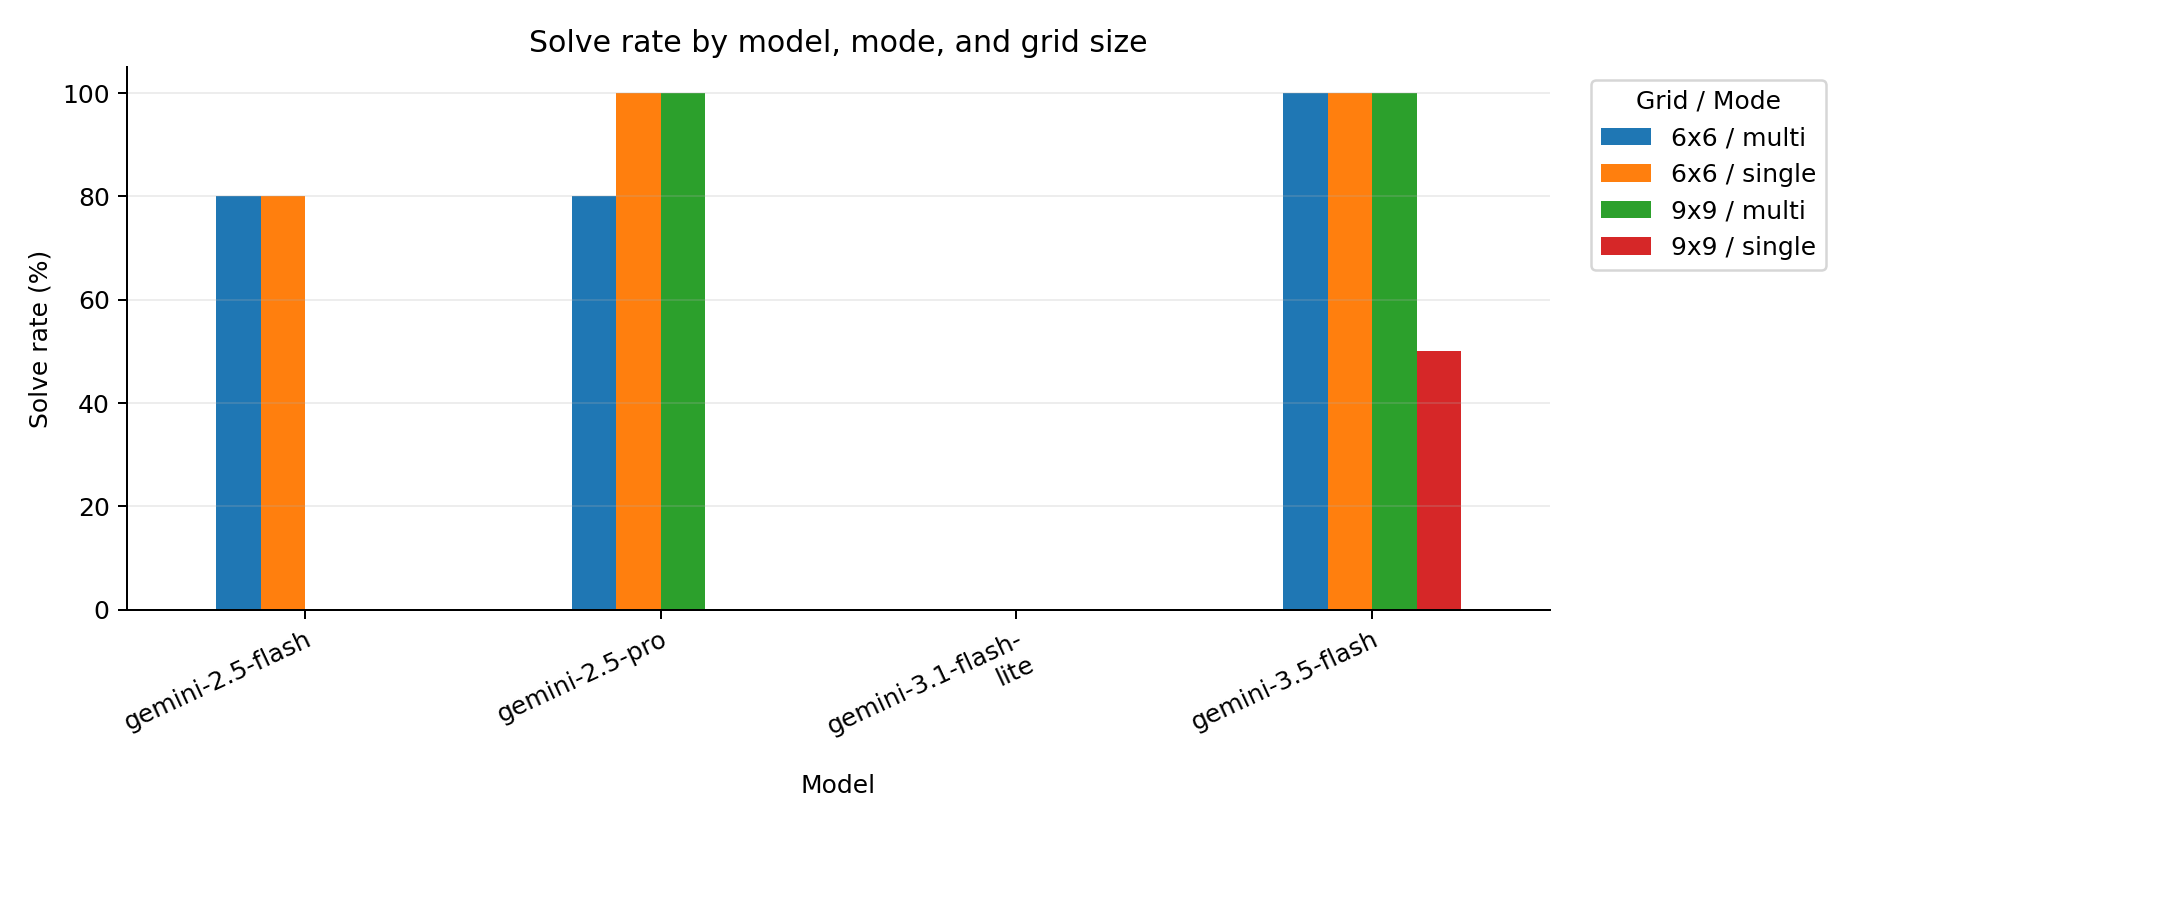
\includegraphics[width=0.95\textwidth]{../cs106/evaluation/eval_outputs/solve_rate_by_model_mode_size.png}}
    {\placeholderfigure{Thiếu file solve\_rate\_by\_model\_mode\_size.png}}
  \caption{Solve rate theo model, mode và kích thước lưới}
\end{figure}

\manualindent%
Kết quả cho thấy 6x6 easy chưa đủ khó để phân tách hoàn toàn các model mạnh: Gemini 2.5 Pro và Gemini 3.5 Flash đều đạt 100\% ở single-prompt; Gemini 3.5 Flash đạt 100\% ở multi-step. Ngược lại, 9x9 hard làm khác biệt rõ hơn: single-prompt hầu hết thất bại, nhưng multi-step giúp hai model mạnh hơn giải đúng toàn bộ 2 bài.

\section{Kết quả single-prompt}

\manualindent%
Single-prompt thể hiện tốt ở 6x6 nhưng giảm mạnh ở 9x9. Ở 6x6, Gemini 2.5 Pro và Gemini 3.5 Flash đều đạt 5/5, Gemini 2.5 Flash đạt 4/5, còn Gemini 3.1 Flash Lite fail toàn bộ. Ở 9x9, chỉ Gemini 3.5 Flash giải được 1/2 bài; các model còn lại đều 0/2.

\manualindent%
Điều này cho thấy một prompt duy nhất có thể đủ cho lưới nhỏ, nhưng khi số ô và số ràng buộc tăng, việc yêu cầu mô hình lập kế hoạch và trả về toàn bộ grid trong một lần trở nên kém ổn định. Khi single-prompt fail, output thường là một grid hoàn chỉnh nhưng sai một hoặc nhiều ô; do đó lỗi chính được phân loại là Incorrect Solution.

\section{Kết quả multi-step}

\manualindent%
Multi-step giúp quan sát quá trình suy luận rõ hơn. Ở 6x6, Gemini 3.5 Flash đạt 5/5, Gemini 2.5 Flash và Gemini 2.5 Pro đạt 4/5, còn Gemini 3.1 Flash Lite fail toàn bộ. Ở 9x9, sự khác biệt trở nên rõ rệt: Gemini 2.5 Pro và Gemini 3.5 Flash đạt 2/2, trong khi Gemini 2.5 Flash và Gemini 3.1 Flash Lite đều không giải được bài nào.

\begin{figure}[H]
  \centering
  \IfFileExists{../cs106/evaluation/eval_outputs/multi_average_correct_placements.png}
    {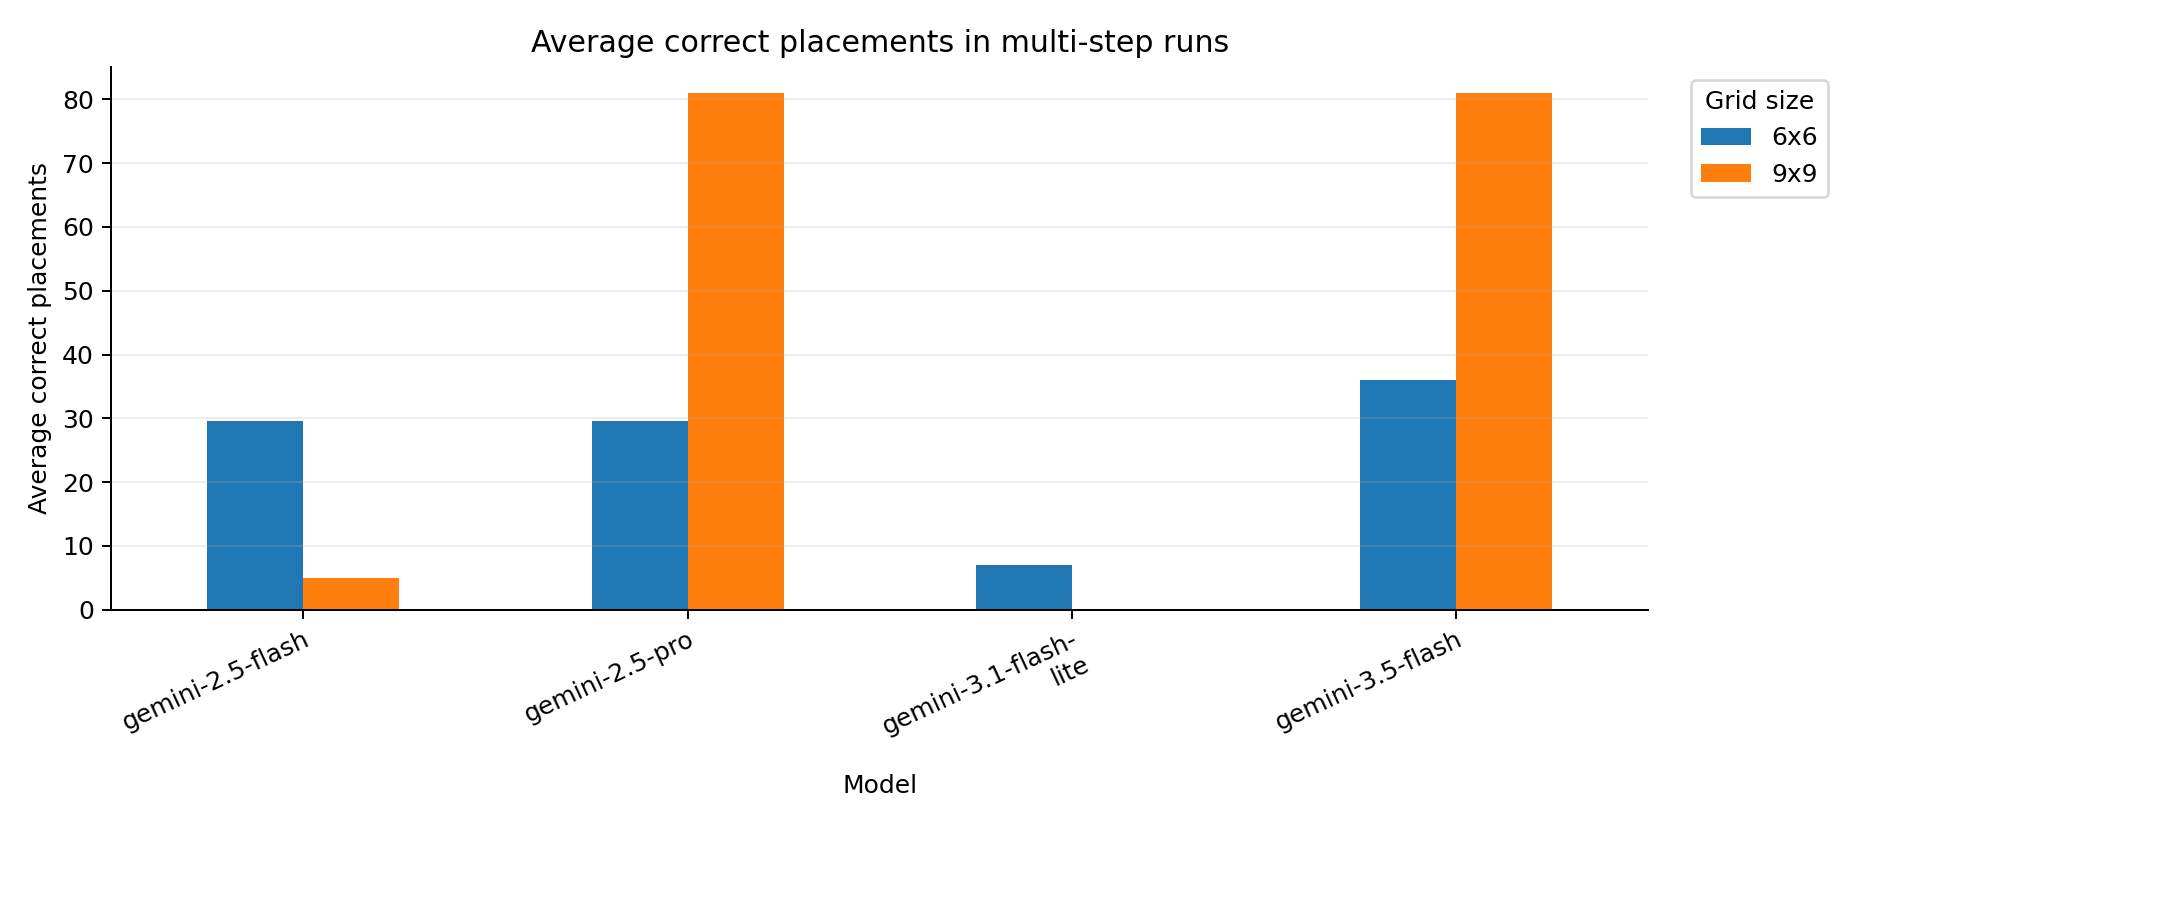
\includegraphics[width=0.9\textwidth]{../cs106/evaluation/eval_outputs/multi_average_correct_placements.png}}
    {\placeholderfigure{Thiếu file multi\_average\_correct\_placements.png}}
  \caption{Average correct placements trong multi-step}
\end{figure}

\manualindent%
Average correct placements cung cấp thông tin sâu hơn solve rate. Với 9x9 multi-step, Gemini 2.5 Flash có solve rate 0\% nhưng vẫn đạt trung bình 5.0/81 correct placements; Gemini 3.1 Flash Lite cũng 0\% nhưng chỉ đạt 0.0/81. Điều này cho thấy hai model cùng fail nhưng mức độ tiến triển khác nhau.

\section{Kết quả theo từng puzzle}

\begin{figure}[H]
  \centering
  \IfFileExists{../cs106/evaluation/eval_outputs/per_puzzle_outcome_heatmap.png}
    {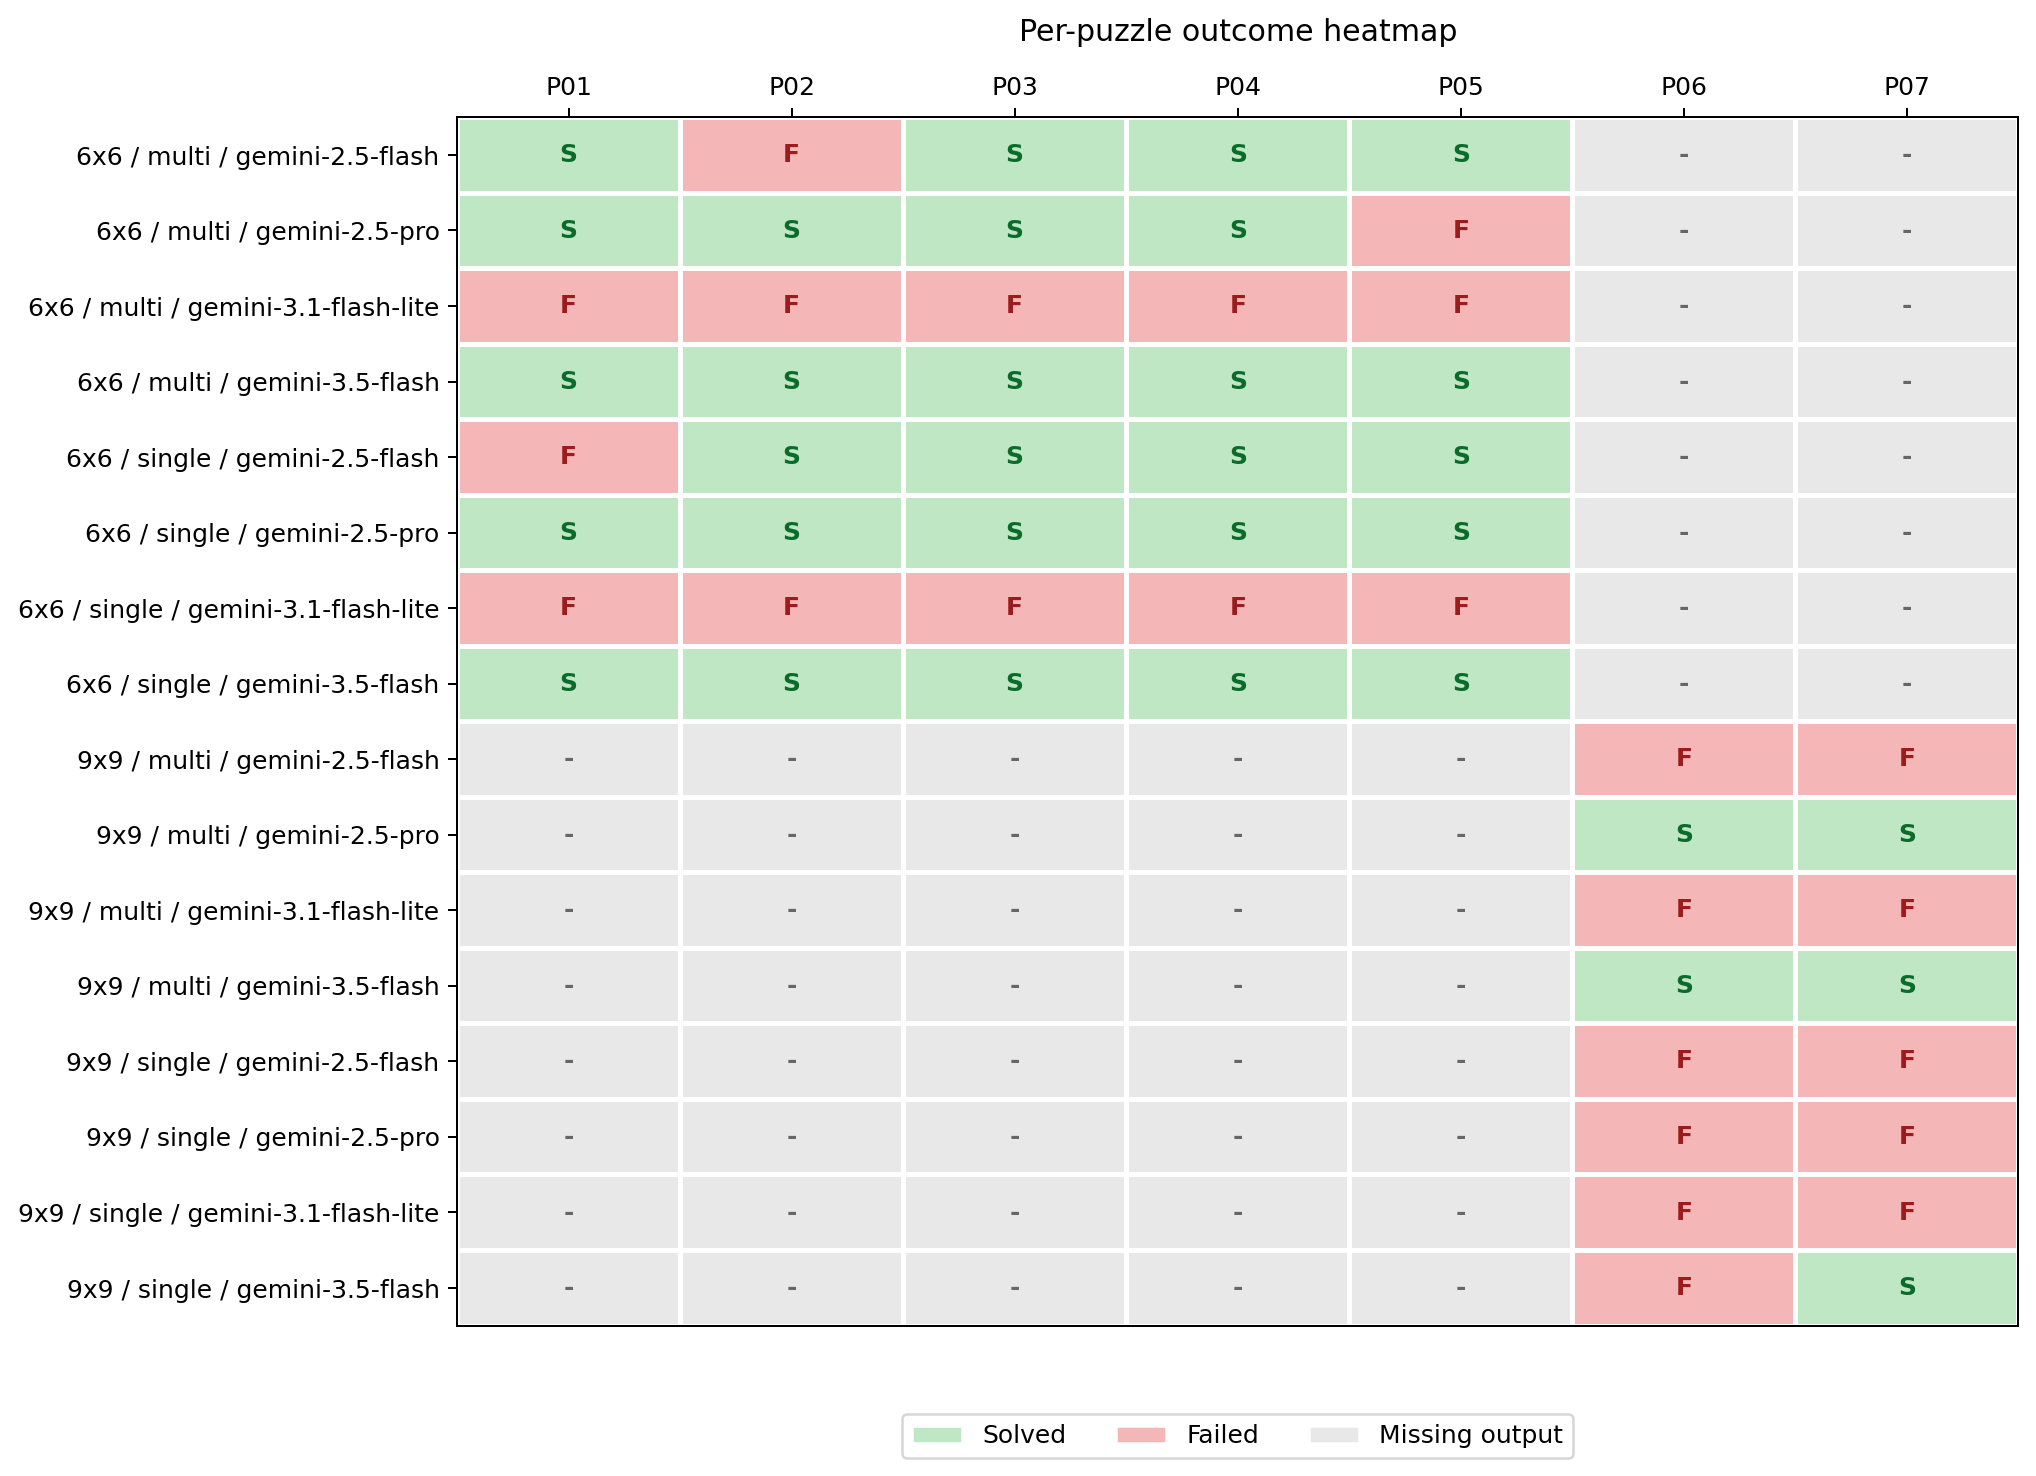
\includegraphics[width=0.95\textwidth]{../cs106/evaluation/eval_outputs/per_puzzle_outcome_heatmap.png}}
    {\placeholderfigure{Thiếu file per\_puzzle\_outcome\_heatmap.png}}
  \caption{Heatmap outcome theo từng puzzle}
\end{figure}

\manualindent%
Ở 6x6, lỗi của Gemini 2.5 Flash và Gemini 2.5 Pro không trùng nhau hoàn toàn: Gemini 2.5 Flash fail ở một puzzle trong multi-step, còn Gemini 2.5 Pro fail ở một puzzle khác. Điều này cho thấy khác biệt không chỉ nằm ở tổng solve rate mà còn nằm ở kiểu puzzle và điểm suy luận làm model sai. Ở 9x9, hai model mạnh đều giải được cả hai bài trong multi-step, trong khi hai model yếu hơn bị kẹt với No Certain Move.

\section{Phân tích lỗi}

\begin{table}[H]
  \centering
  \caption{Tóm tắt error type chính}
  \small
  \begin{tabularx}{\textwidth}{p{3.5cm}p{4.5cm}X}
    \toprule
    Error type & Xuất hiện chính ở đâu & Ý nghĩa \\
    \midrule
    Incorrect Solution & Single-prompt và một số multi-step 6x6 & Model đưa ra grid hoặc bước đi sai so với nghiệm chuẩn \\
    No Certain Move & Multi-step 9x9 của model yếu hơn & Model không tìm được bước chắc chắn để tiếp tục, dù chưa điền sai trực tiếp \\
    Success & Các phiên giải đúng hoàn toàn & Grid cuối khớp nghiệm chuẩn \\
    \bottomrule
  \end{tabularx}
\end{table}

\begin{figure}[H]
  \centering
  \IfFileExists{../cs106/evaluation/eval_outputs/error_type_summary.png}
    {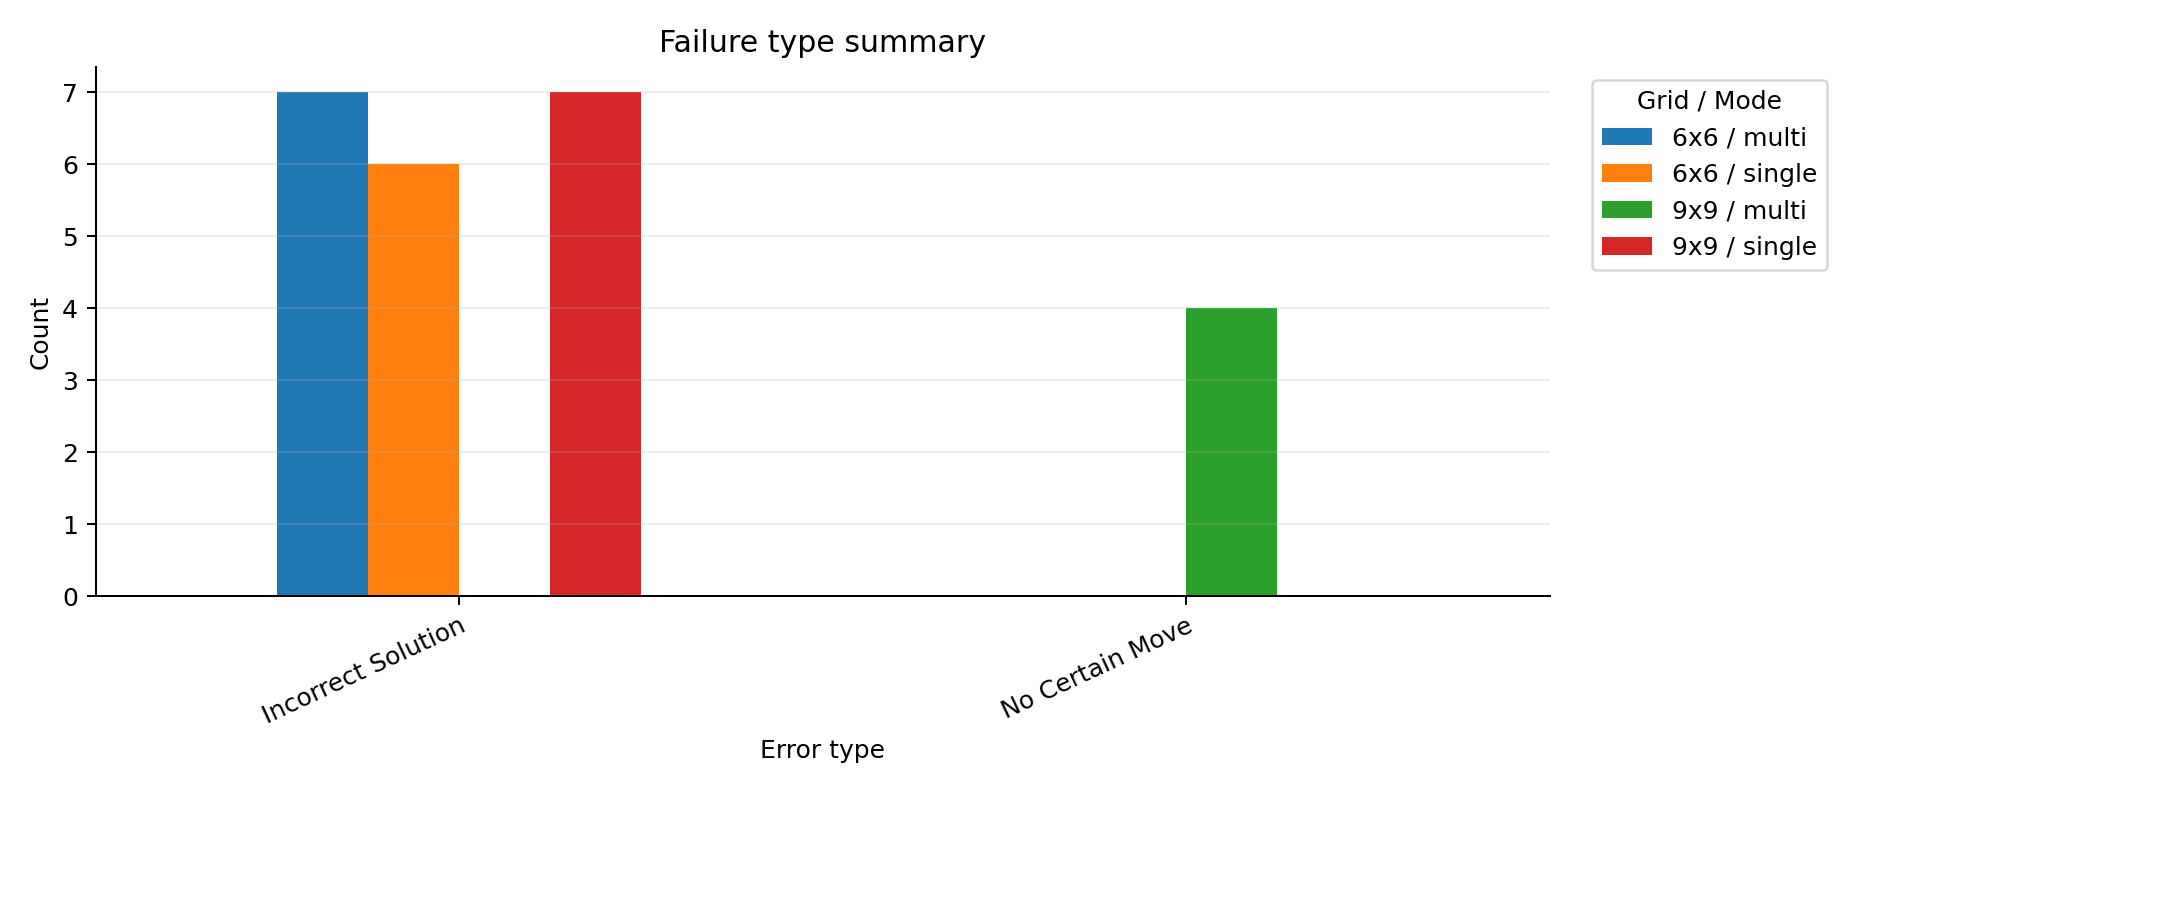
\includegraphics[width=0.88\textwidth]{../cs106/evaluation/eval_outputs/error_type_summary.png}}
    {\placeholderfigure{Thiếu file error\_type\_summary.png}}
  \caption{Tổng hợp error type theo grid/mode}
\end{figure}

\manualindent%
Incorrect Solution phản ánh tình huống mô hình tự tin đưa ra đáp án nhưng đáp án không khớp nghiệm chuẩn. No Certain Move lại khác: mô hình không nhất thiết điền sai, nhưng bị kẹt vì không thể xác định bước chắc chắn. Trong bối cảnh đánh giá reasoning, No Certain Move là lỗi có giá trị phân tích vì nó cho thấy giới hạn của mô hình trong việc tìm break-in hoặc tiếp tục lan truyền ràng buộc.

\section{Thời gian và chi phí thực nghiệm}

\manualindent%
Thời gian chạy được ghi nhận đầy đủ cho single-prompt. Ở 6x6 single-prompt, Gemini 3.5 Flash có thời gian trung bình thấp nhất trong log hiện tại, khoảng 27.57 giây/puzzle; Gemini 2.5 Flash khoảng 169.65 giây/puzzle; Gemini 2.5 Pro khoảng 106.13 giây/puzzle. Ở 9x9 single-prompt, thời gian tăng lên rõ, đặc biệt Gemini 3.5 Flash trung bình khoảng 311.04 giây/puzzle.

\begin{figure}[H]
  \centering
  \IfFileExists{../cs106/evaluation/eval_outputs/average_time_seconds_by_model_mode_size.png}
    {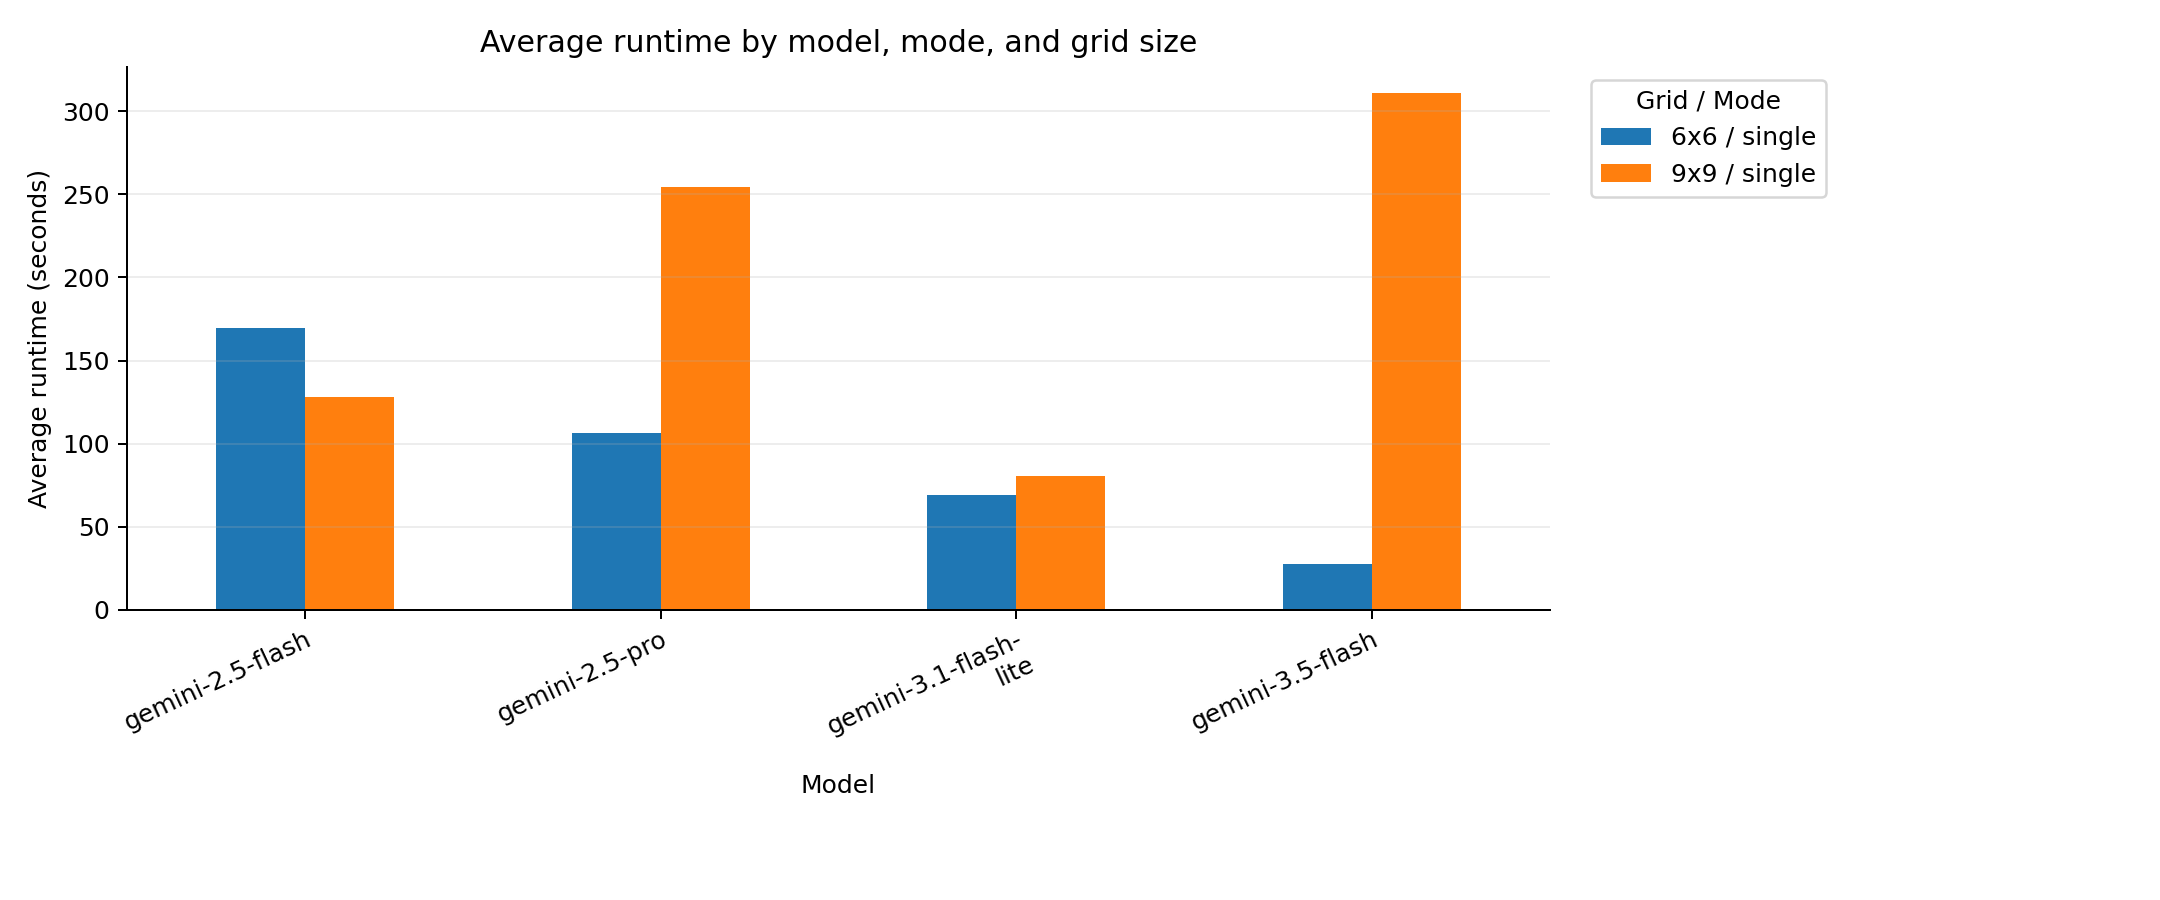
\includegraphics[width=0.92\textwidth]{../cs106/evaluation/eval_outputs/average_time_seconds_by_model_mode_size.png}}
    {\placeholderfigure{Thiếu file average\_time\_seconds\_by\_model\_mode\_size.png}}
  \caption{Thời gian trung bình cho các lượt single-prompt có ghi log}
\end{figure}

\manualindent%
Đối với multi-step, file tổng hợp hiện tại chưa lưu đầy đủ thời gian từng phiên, nên báo cáo không đưa ra so sánh định lượng chính thức về thời gian multi-step. Tuy nhiên, về mặt thiết kế, chi phí multi-step tăng theo số ô: 6x6 có 36 ô, còn 9x9 có 81 ô; nếu mỗi ô cần một lượt analysis và một lượt fill, số lượt gọi tối thiểu có thể tăng từ 72 lên 162 cho mỗi puzzle. Đây là lý do nhóm chỉ chạy 2 bài 9x9 hard.

\section{So sánh với paper gốc}

Kết quả của nhóm phù hợp với các nhận định chính của Sudoku-Bench:

\begin{itemize}
  \item Sudoku variants là benchmark tốt vì kết quả có thể validate khách quan.
  \item Các puzzle lớn và nhiều ràng buộc khó hơn rõ rệt.
  \item LLM có thể sinh reasoning nghe hợp lý nhưng vẫn sai về mặt hình thức.
  \item Multi-step không chỉ cải thiện solve rate trong một số trường hợp mà còn giúp quan sát quá trình suy luận và phân tích lỗi.
\end{itemize}

Điểm khác biệt là quy mô của nhóm nhỏ hơn nhiều so với paper. Vì vậy, kết quả không nhằm khẳng định model nào tốt nhất một cách tổng quát, mà nhằm tái hiện logic đánh giá của paper trong phạm vi đồ án và minh họa rõ cách một benchmark reasoning có thể được triển khai.

% =========================
% Chapter 6
% =========================
\chapter{KẾT LUẬN VÀ HƯỚNG PHÁT TRIỂN}

\section{Kết luận}

\manualindent%
Đồ án đã hoàn thành mục tiêu tái hiện rút gọn bài báo Sudoku-Bench trên biến thể Killer Sudoku. Nhóm đã xây dựng pipeline từ dữ liệu JSON đến prompt, API call, parser, validator, logger và evaluation notebook. Thực nghiệm được mở rộng từ 2 model ban đầu lên 4 model Gemini, bao gồm cả single-prompt và multi-step trên 6x6 và 9x9.

\manualindent%
Kết quả cho thấy single-prompt có thể hoạt động tốt ở 6x6 với các model mạnh, nhưng giảm mạnh ở 9x9. Multi-step cho kết quả nổi bật hơn ở 9x9: Gemini 2.5 Pro và Gemini 3.5 Flash đạt 2/2, trong khi các model yếu hơn bị kẹt ở No Certain Move. Điều này cho thấy việc chia quá trình suy luận thành từng bước có thể giúp model mạnh duy trì trạng thái tốt hơn, đồng thời tạo log để phân tích lỗi.

\manualindent%
Quan trọng hơn, đồ án cho thấy validator là thành phần bắt buộc khi đánh giá LLM trên bài toán ràng buộc. Reasoning bằng ngôn ngữ tự nhiên không đủ để kết luận lời giải đúng; cần đối chiếu với nghiệm chuẩn và lưu lại từng bước.

\section{Hạn chế}

Đồ án vẫn còn một số hạn chế:

\begin{itemize}
  \item Dataset nhỏ hơn nhiều so với bài báo gốc, chỉ gồm 7 puzzle.
  \item Nhóm chỉ tập trung Killer Sudoku, chưa thử các variant khác như Arrow, Thermometer hoặc Knight's Move.
  \item Các mô hình đều thuộc hệ sinh thái Gemini, chưa so sánh với GPT, Claude hoặc model mã nguồn mở.
  \item 9x9 chỉ có 2 puzzle, chưa đủ để kết luận tổng quát về toàn bộ lớp 9x9 hard.
  \item Multi-step tốn nhiều lượt gọi API và file tổng hợp hiện tại chưa lưu đầy đủ thời gian cho từng phiên multi-step.
  \item Prompt/cheat sheet có ảnh hưởng lớn đến kết quả, nên một phần khác biệt có thể đến từ thiết kế prompt chứ không chỉ từ năng lực model.
\end{itemize}

\section{Hướng phát triển}

Trong tương lai, có thể mở rộng đồ án theo các hướng sau:

\begin{itemize}
  \item Tăng số lượng puzzle 6x6 và 9x9, đồng thời chạy lặp nhiều lần để giảm nhiễu do sampling.
  \item Thử thêm nhiều Sudoku variants ngoài Killer Sudoku.
  \item Chuẩn hóa hệ thống logging để ghi đầy đủ thời gian, số token và chi phí API cho multi-step.
  \item So sánh thêm các model ngoài Gemini để tăng tính khách quan.
  \item Bổ sung các metric như first wrong step, candidate consistency và cage-level violation.
  \item Nghiên cứu hướng neuro-symbolic: LLM đề xuất reasoning, solver hình thức kiểm tra hoặc phản hồi ràng buộc.
\end{itemize}

\section{Bài học rút ra}

\manualindent%
Qua đồ án, nhóm nhận thấy việc đánh giá LLM trên bài toán logic không thể chỉ dựa trên câu trả lời cuối hoặc phần giải thích tự nhiên. Cần thiết kế dữ liệu có ground truth, định dạng output có thể parse, validator độc lập và các metric phản ánh cả quá trình. Sudoku-Bench là một ví dụ tốt cho cách xây dựng benchmark reasoning: bài toán đủ dễ để mô tả bằng ngôn ngữ, nhưng đủ chặt để phát hiện sai sót hình thức của mô hình.

% =========================
% References
% =========================
\begin{thebibliography}{9}

\bibitem{sudoku-bench}
Jeffrey Seely, Yuki Imajuku, Tianyu Zhao, Edoardo Cetin, and Llion Jones.
\textit{Sudoku-Bench: Evaluating Creative Reasoning with Sudoku Variants}.
Sakana AI, arXiv:2505.16135, 2025.

\bibitem{russell-norvig}
Stuart Russell and Peter Norvig.
\textit{Artificial Intelligence: A Modern Approach}.
Pearson, 4th edition, 2020.

\bibitem{vaswani}
Ashish Vaswani, Noam Shazeer, Niki Parmar, Jakob Uszkoreit, Llion Jones, Aidan N. Gomez, Lukasz Kaiser, and Illia Polosukhin.
\textit{Attention Is All You Need}.
Advances in Neural Information Processing Systems, 2017.

\end{thebibliography}

\end{document}
